

\section{Problem 3}
\label{part3}
Consider the "bow-tie" graph in the Broder et al. paper (fig 9):
url{http://www9.org/w9cdrom/160/160.html}\\


\noindent Now consider the following graph:
    \begin{verbatim}
    A --> B
    B --> C
    C --> D
    C --> A
    C --> G
    E --> F
    G --> C
    G --> H
    I --> H
    I --> J
    I --> K
    J --> D
    L --> D
    M --> A
    M --> N
    N --> D
     \end{verbatim}
    For the above graph, give the values for:\\
IN: \\
SCC: \\
OUT: \\
Tendrils: \\
Tubes: \\
Disconnected:

\subsection{Solution}
\begin{enumerate}
\item First the graph should be drawn in order to figure out which nodes fall under which category. 
\item The values for the given graph are:
\begin{verbatim}
IN: M
SCC: A,B,C,G,
OUT: D,H
In Tendril: None
Out Tendril : L,K,I,J
Tubes: M-->N-->D
Disconnected: E-->F
\end{verbatim}

\end{enumerate}

\newpage
\subsection{Results}
\begin{figure}[ht]    
    \begin{center}
        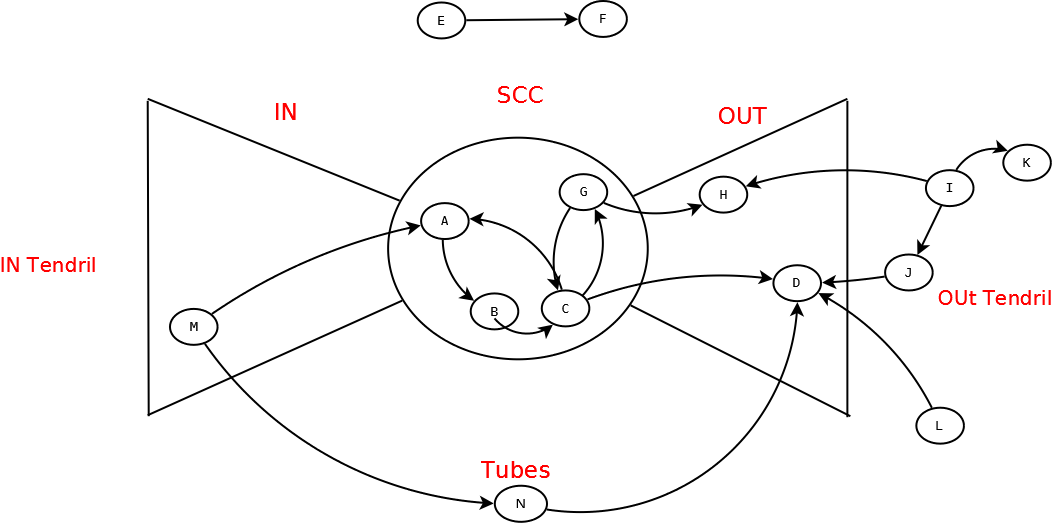
\includegraphics[scale=0.30]{part3.png}
        \caption{BowTie Graph}
        \label{fig:X-distribution}
    \end{center}
\end{figure}
\subsection{Explanation}
\begin{enumerate}
\item Its pretty clear that the node E and F are not at all connected to the any part of the graph, they fall under Disconnected. 
\item According to the definition of IN,i:e any vertex in IN can be connected to or from any other node in IN, and can be connected to any node in SCC but never from anywhere else, that leaves nodes M in IN.
\item For OUT, the nodes in OUT can be linked from any node in SCC but never the other way. There can never be any node linked from OUT.So that leaves node D,H in OUT.
\item For SCC, the node in scc can be linked from In and linked to OUT. The other feature of SCC is that the nodes in SCC can link to any other node in SCC, that leaves node A,B,C,G.
\item For tubes, the nodes which are linked from IN to Out fall under Tubes. These can not connect to any nodes in SCC, that leaves Nodes N Under Tubes.
\item Tendrils: Tendrils are two types In Tendrils and Out Tendrils. The In Tendrils are the nodes that can never connect to any other nodes in SCC,tubes or OUT
\item Out Tendrils: Out Tendrils are the tendril which can never connect to any other nodes other than the nodes in OUT. That leaves L,K,I,J as Out Tendrils. 
\end{enumerate}
